\documentclass[12pt, a4paper, oneside]{ctexart}
\usepackage{amsmath, amsthm, amssymb, bm, color, framed, graphicx, hyperref, mathrsfs, geometry}
\usepackage{algorithm, algorithmicx, algpseudocode, pdfpages, dsfont}

\title{\textbf{机器学习第三次作业}}
\author{汪隽立\ 计14\ 2021012957}
\date{\today}
\linespread{1.5}
\definecolor{shadecolor}{RGB}{241, 241, 255}
\newcounter{problemname}
\newenvironment{problem}[1]{\begin{shaded}\par\noindent\textbf{题目 #1. }}{\end{shaded}\par}
\newenvironment{solution}[1]{\par\noindent\textbf{解答 #1. }\par}{\par}
\newenvironment{note}{\par\noindent\textbf{题目\arabic{problemname}的注记. }}{\par}

\geometry{a4paper,scale=0.8}
\begin{document}

\maketitle

\begin{solution}{2.1.1}
    在第一次选择划分特征时,因为$x_2$,$x_3$的信息增益都为$0$,故选择$x_1$。第一次划分以后,对于左节点,其经验熵为
    $$
        H(D)=-\frac{2}{3}\log\frac{2}{3}-\frac{1}{3}\log\frac{1}{3}=0.918
    $$
    对于左节点的第二步划分,选择$x_2$,$x_3$的信息增益都为
    $$
        IG = H(D)-\left[\frac{2}{3}(-\frac{1}{2}\log\frac{1}{2}-\frac{1}{2}\log\frac{1}{2})+\frac{1}{3}\times0\right]=0.252
    $$
    也就是说,第二步无论选择$x_2$还是$x_3$作为划分特征,总会有一个叶节点包括两个$y$不同的样本,也即这里会有一个样本被分类错误,即$\epsilon\ge\frac{1}{4}$。
    \begin{figure}[htbp]
        \centering
        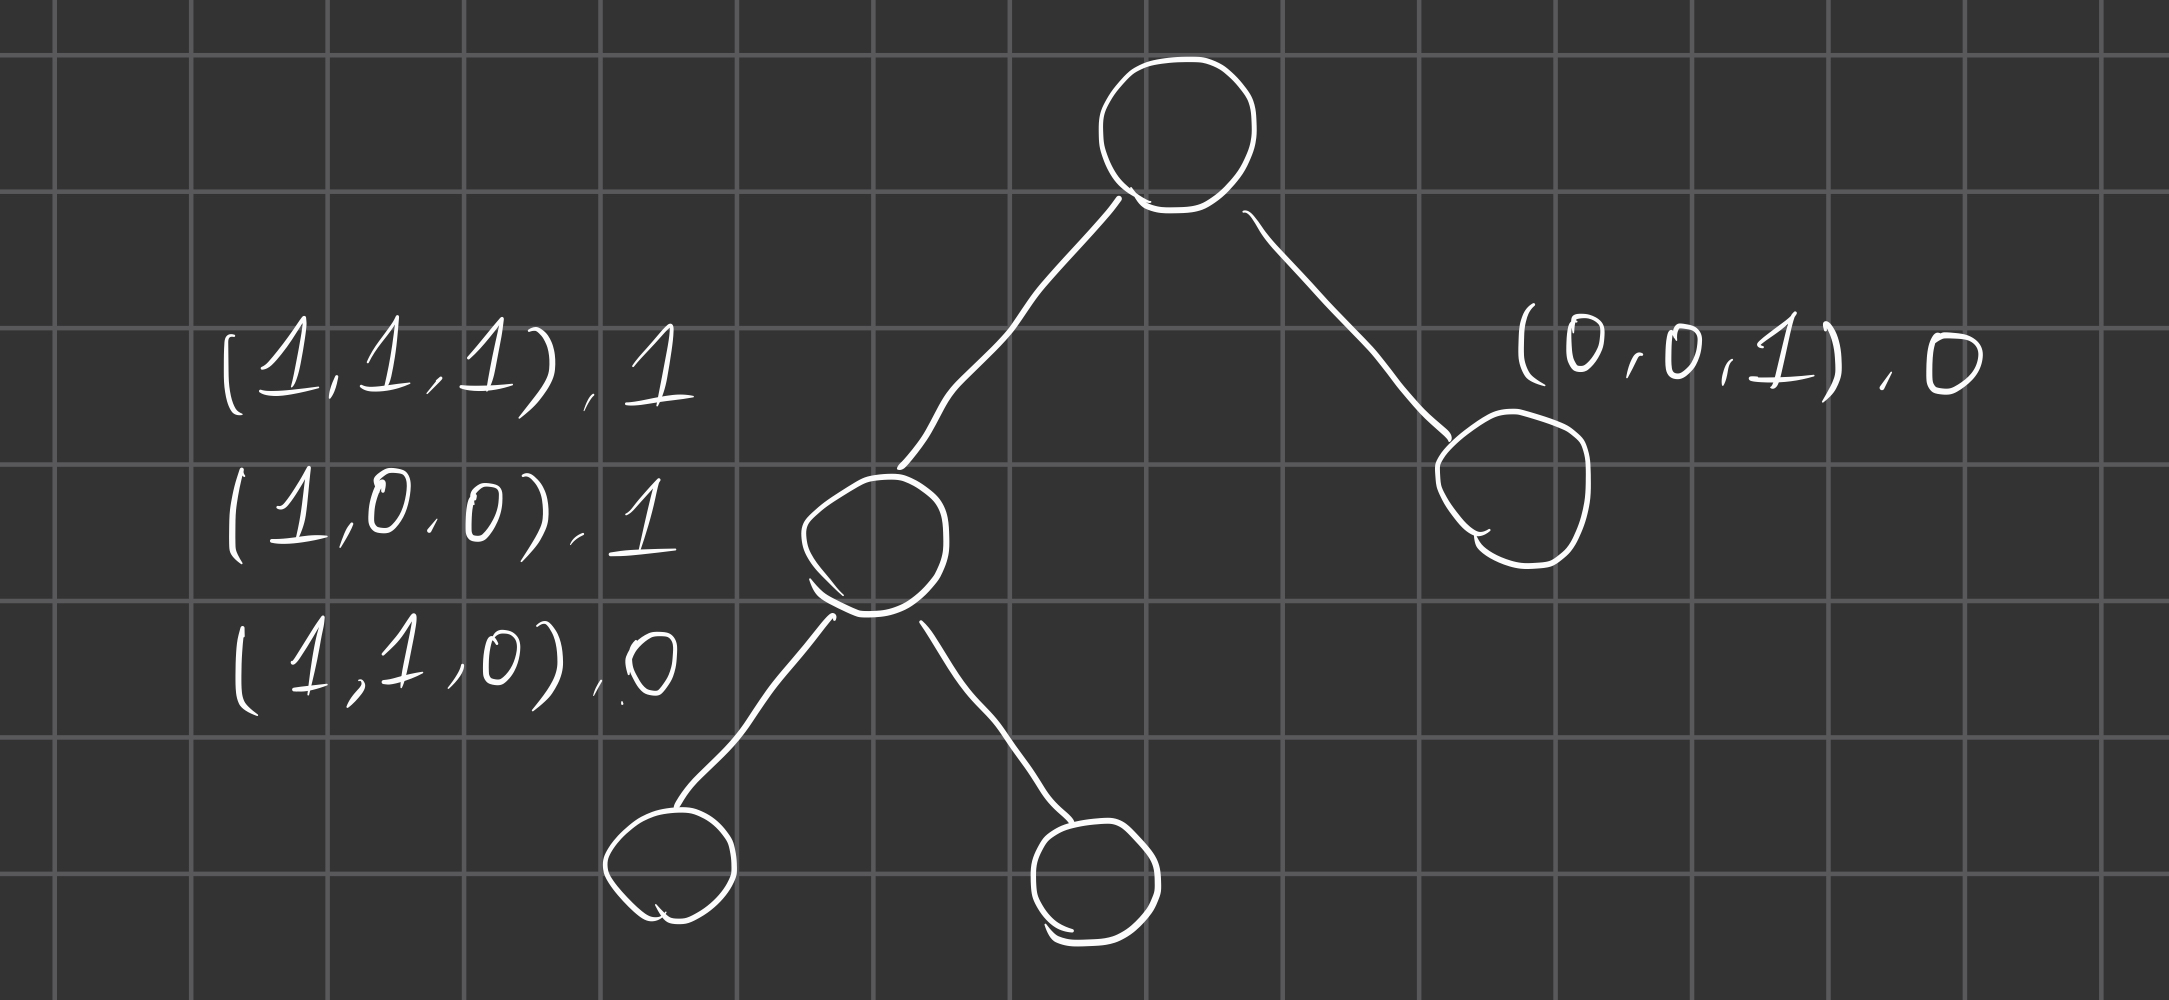
\includegraphics[width=0.5\textwidth]{pic/1.jpeg}
        \caption{Sol 2.1.1}
    \end{figure}
\end{solution}

\begin{solution}{2.1.2}
    如图2所示。
    \begin{figure}[htbp]
        \centering
        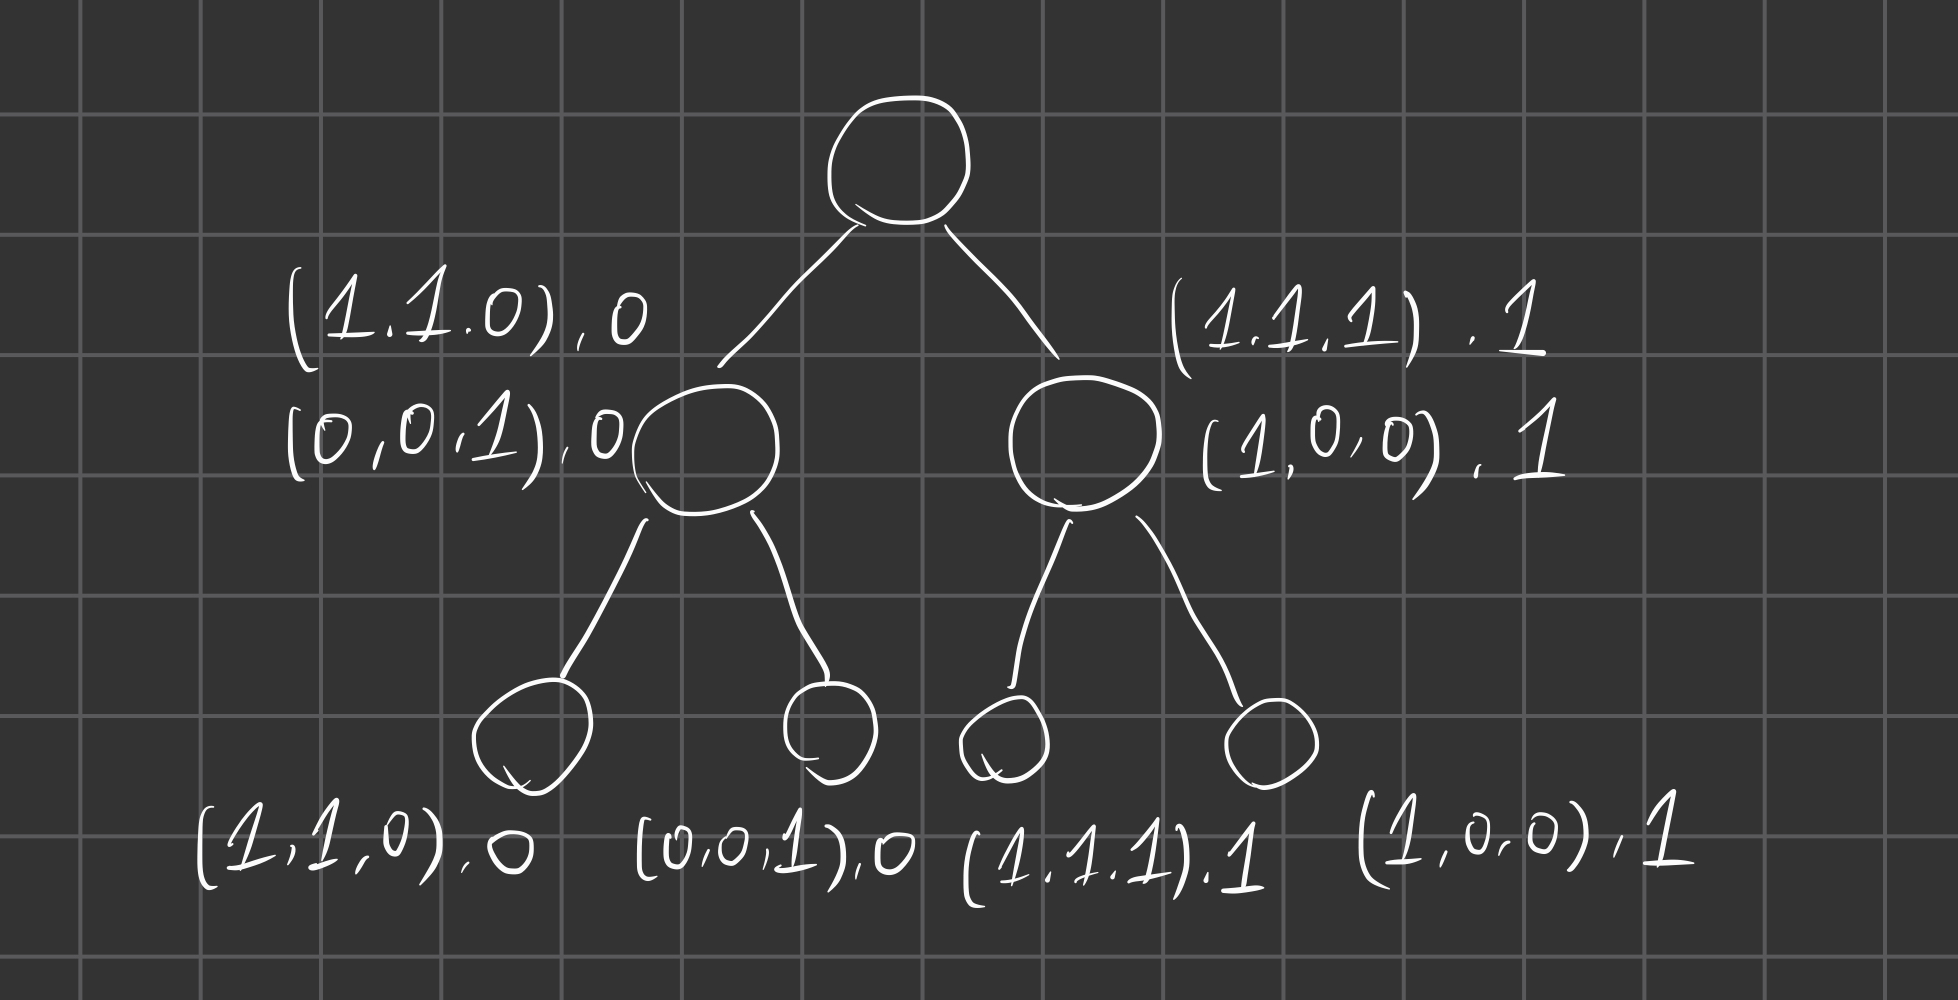
\includegraphics[width=0.5\textwidth]{pic/2.jpeg}
        \caption{Sol 2.1.2}
    \end{figure}
\end{solution}

\begin{solution}{2.2.1}
    $t$个决策树,每个决策树都不选该特征的概率为$(1-\frac{1}{d})^t$。
\end{solution}

\begin{solution}{2.2.2}
    $t$个决策树,每个决策树独立自助$m$个样本。某个样本从未被选中的概率为$(1-\frac{1}{n})^{mt}$。
\end{solution}

\begin{solution}{2.3.5}
    实验结果见图3。\par
    实验过程中,可调整的超参数有min\_sample和max\_depth。在给出的结果中,可以看出当max\_depth为4时,模型就已经较好地学习到了数据的分布。这时,随着max\_depth的增加,模型的泛化能力不再增加,对于过拟合的现象不能很好地解决。\par
    而适当增加min\_sample,可以增加模型的泛化能力。例如当min\_sample变为30时,分类问题的结果变成了图4:
    \begin{figure}[htbp]
        \centering
        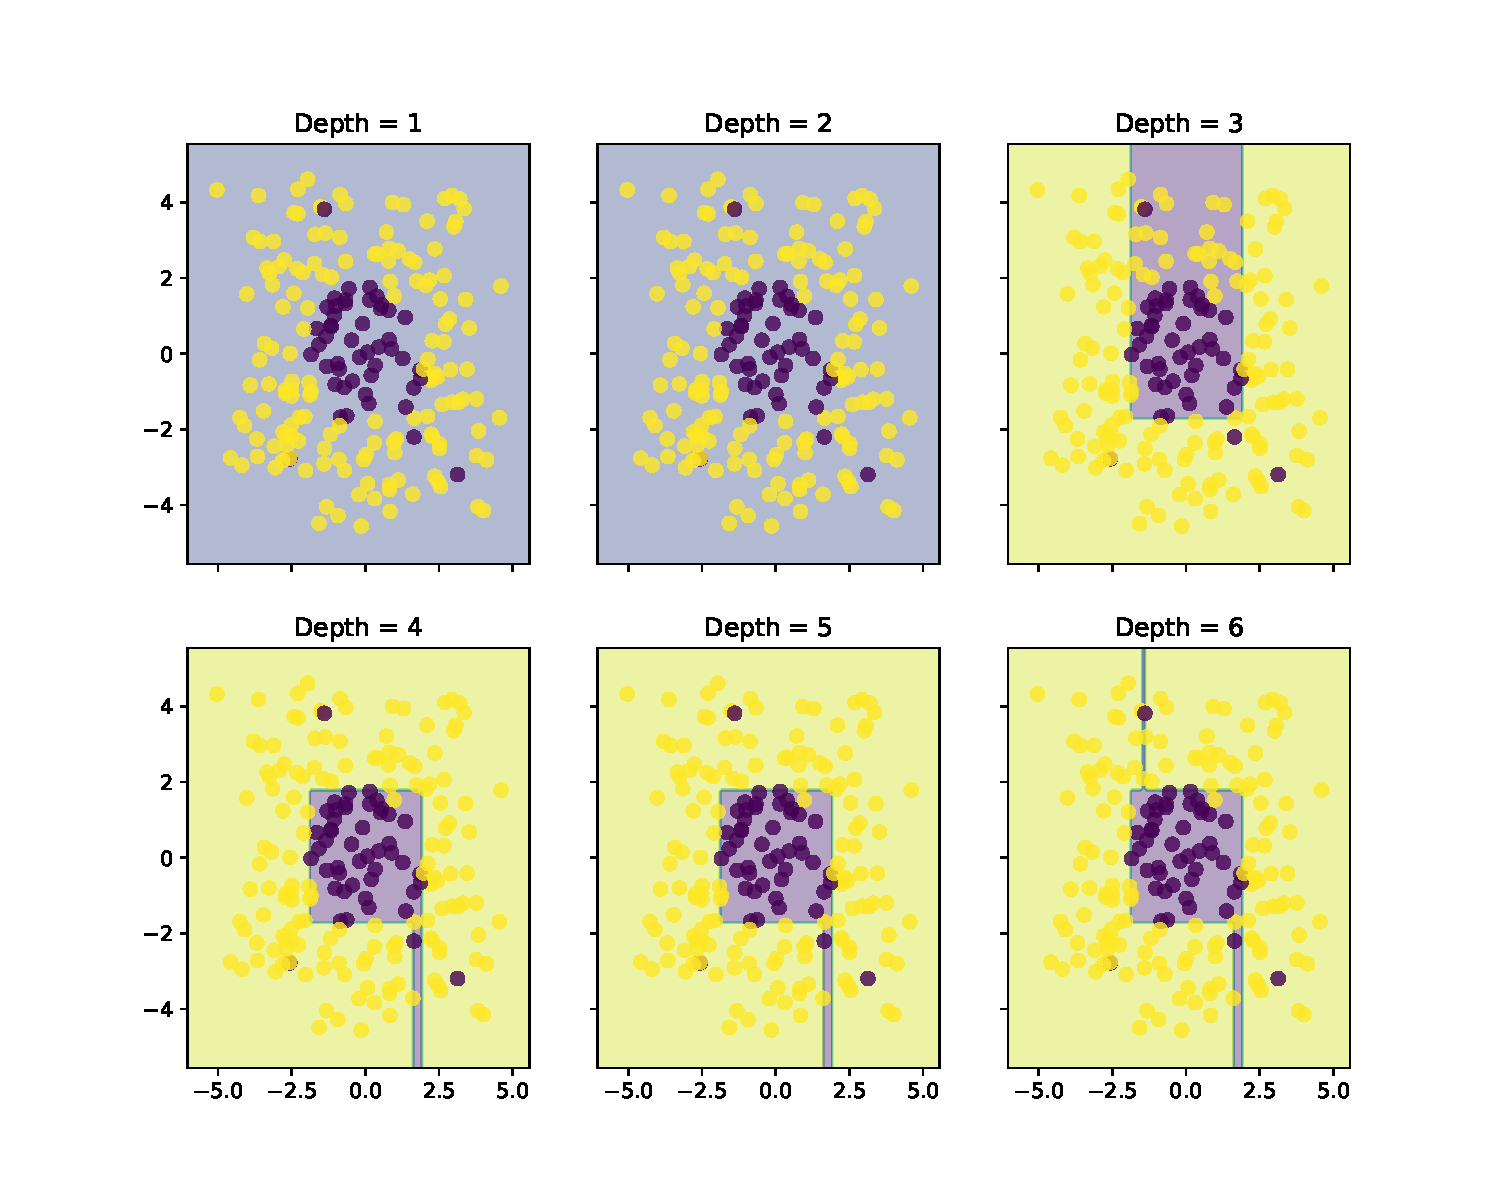
\includegraphics[width=.9\textwidth]{pdf/DT_entropy.pdf}
        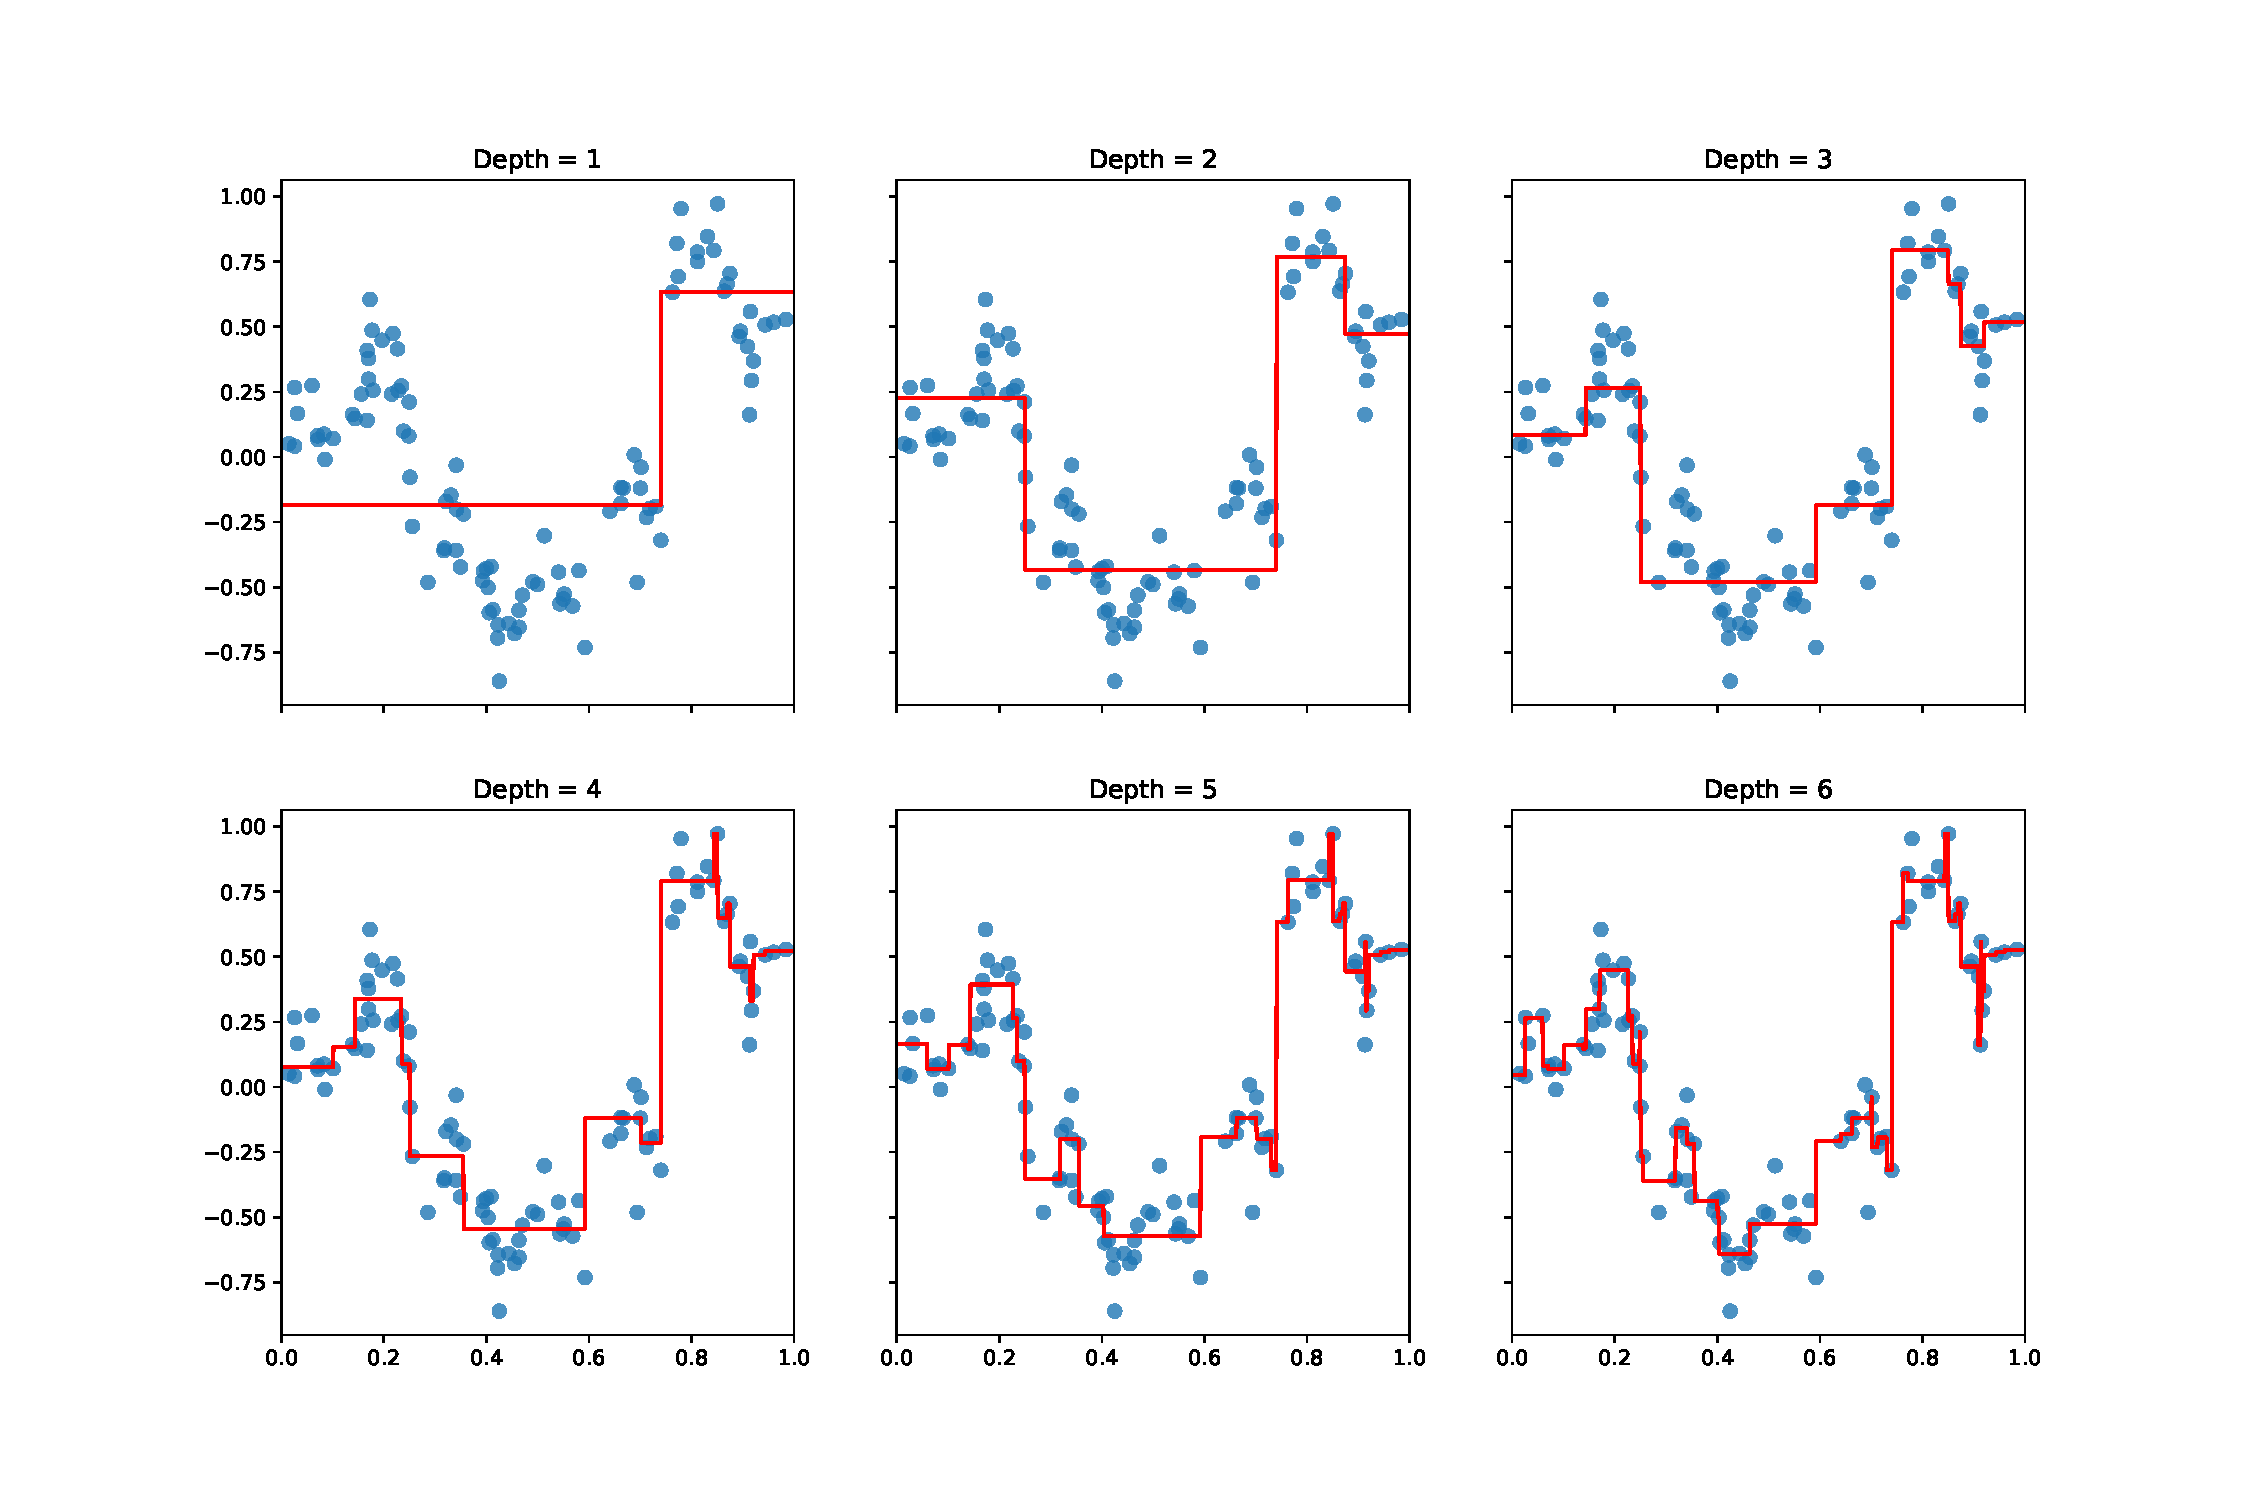
\includegraphics[width=.9\textwidth]{pdf/DT_regression.pdf}
        \caption{Sol 2.3.5}
    \end{figure}

    \begin{figure}[htbp]
        \centering
        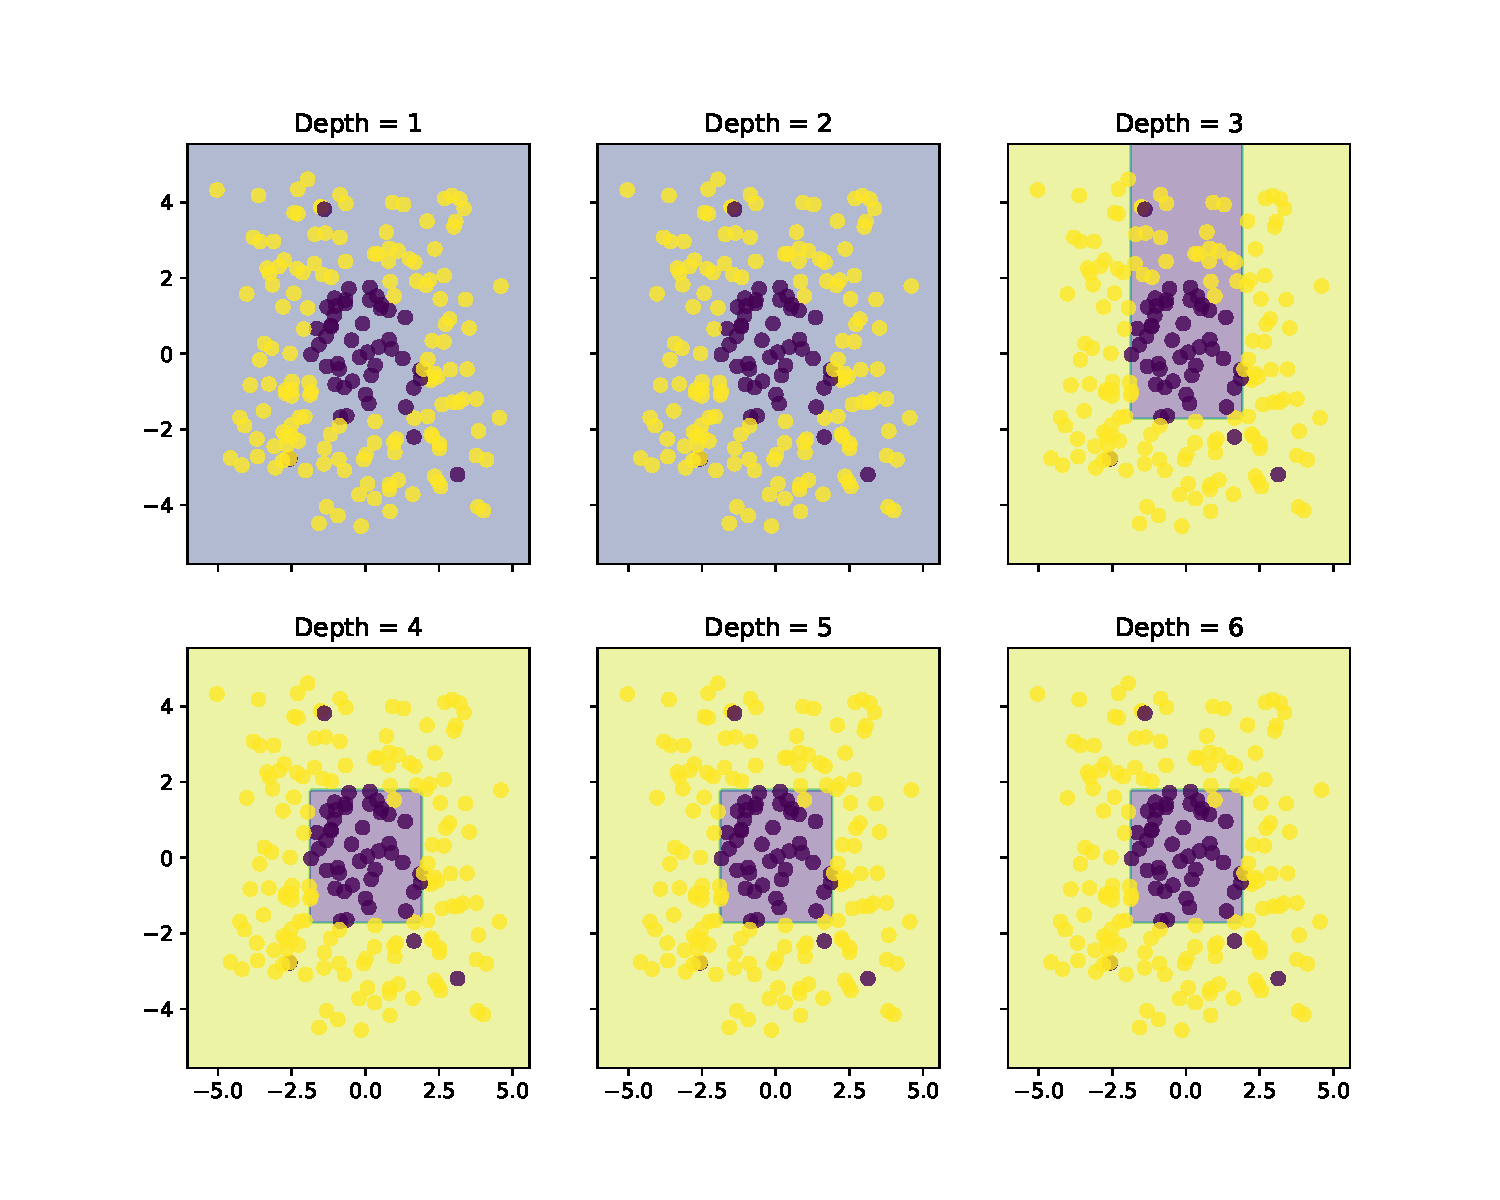
\includegraphics[width=.9\textwidth]{pdf/1.pdf}
        \caption{min\_sample=30}
    \end{figure}

\end{solution}

\begin{solution}{3.1.1}
    首先证明$G$在$x=0$处可导。$\lim_{x\to0^+}\frac{G(x)-1}{x}=1$,$\lim_{x\to0^-}\frac{G(x)-1}{x}=\lim_{x\to0^-}\frac{e^x-1}{x}=1$。故$G^\prime(0)=1$。又$G$在除了$x=0$处处可导,故$G$处处可导。\par
    \begin{align}
        G^\prime(x) = 
        \begin{cases}
            1 & x>1\\
            e^x & x\le0
        \end{cases}
        \nonumber
    \end{align}
    因为$G^\prime$单调递增,故$G$是$\mathbb{R}$上的凸函数。
\end{solution}

\begin{solution}{3.1.2}
    定义$D_t(i)Z_t=G(-y_i\sum_{j=1}^{N}\bar{\alpha_{t,j}} h_j(x_i))$,$Z_t$是归一化因子。那么:
    $$
    \epsilon_t(h)=\sum_{i=1}^{m}D_t(i)\mathds{1}_{\left[ h(x_i)\neq y_i\right]}
    $$。以下证明其合理性:\par
    利用坐标下降的方法,我们可以类似地得到:
    \begin{align}
        F^\prime(\bar{\alpha_{t}}, e_k)=&\lim_{\eta\to0}\frac{F(\bar{\alpha_{t}}+\eta e_k)-F(\bar{\alpha_{t}})}{\eta}\nonumber \\
        =&\frac{1}{m}\sum_{i=1}^{m}y_i h_k(x_i)G(-y_i \sum_{j=1}^{N}\bar{\alpha_{t,j}} h_j(x_i))\nonumber \\
        =& -\frac{Z_t}{m}\left[ \sum_{i=1}^{m} D_t(i)\mathds{1}_{\left[ y_i h_k(x_i)=+1 \right]} - \sum_{i=1}^{m} D_t(i)\mathds{1}_{\left[ y_i h_k(x_i)=-1 \right]} \right]\nonumber \\
        =& (2\epsilon_{t, k}-1)\frac{Z_t}{m}\nonumber
    \end{align}
    也就是说,在新的Boosting算法中,我们找的依然是使得坐标下降最快的那个$h_k$。
\end{solution}

\begin{solution}{3.2}
    \begin{align}
    \sum_i D_{t+1}(i)\mathds{1}_{[y_i\neq h_t(x_i)]}=&\sum_i \frac{D_t(i)\exp(-\alpha_t y_i h_t(x_i))}{Z_t}\mathds{1}_{[y_i\neq h_t(x_i)]} \nonumber \\
    =&\frac{\exp(\alpha_t)}{Z_t}\epsilon_t \text{\qquad(在上一行中只取$y_i\neq h_t(x_i)$的项)} \nonumber \\
    =&\sqrt{\frac{1-\epsilon_t}{\epsilon_t}} \frac{1}{2\sqrt{\epsilon_t(1-\epsilon_t)}}\epsilon_t \nonumber \\
    =&\frac{1}{2} \nonumber
    \end{align}
    因此,如果第$t+1$步选取的弱分类器和第$t$步的相同,那么说明第$t+1$步时,\textbf{$\mathcal{H}$中的所有分类器至少拥有$\frac{1}{2}$的误差},这与Weak-Learnable的假设矛盾。
\end{solution}

\begin{solution}{3.3}
    根据Adaboost的Empirical Bound: 
    $$
        \hat{R}(h)\leq \exp(-2\gamma T^2)
    $$
    当$T>\frac{\log m}{2\gamma^2}$时,有$\hat{R}(h)<\frac{1}{m}$。又$\hat{R}(h)=\{0, \frac{1}{m}, \frac{2}{m}, \dots, 1\}$,故这时有$\hat{R}(h)=0$。
\end{solution}

\begin{solution}{3.4}
    选择
    $$
    \alpha=\frac{1}{2}\log\frac{1+2\gamma}{1-2\gamma}
    $$
    根据Adaboost的Empirical Bound,有:
    \begin{align}
        Z_t\leq& (1-\epsilon_t)\exp(-\alpha_t)+\epsilon_t\exp(\alpha_t) \nonumber\\
        =&(1-\epsilon_t)\sqrt{\frac{1-2\gamma}{1+2\gamma}}+\epsilon_t\sqrt{\frac{1+2\gamma}{1-2\gamma}} \nonumber\\
        =&(\sqrt{\frac{1+2\gamma}{1-2\gamma}}-\sqrt{\frac{1-2\gamma}{1+2\gamma}})\epsilon_t+\sqrt{\frac{1-2\gamma}{1+2\gamma}} \nonumber\\
        \leq&(\sqrt{\frac{1+2\gamma}{1-2\gamma}}-\sqrt{\frac{1-2\gamma}{1+2\gamma}})(\frac{1}{2}-\gamma)+\sqrt{\frac{1-2\gamma}{1+2\gamma}} \nonumber \\
        =&\sqrt{1-4\gamma^2}\nonumber
    \end{align}
    再利用$\hat{R}(h)\leq \prod_{t=1}^{T} Z_t$,即得$\hat{R}(h)\leq (1-4\gamma^2)^{\frac{T}{2}}$。
\end{solution}

\begin{solution}{3.5.1}
    $$
        h_t=\text{arg}\min_{h\in\mathcal{F}}||h_t+g_t||^2
    $$
    $$
        f_t(x)=f_{t-1}(x)+\alpha_t h_t(x)
    $$
\end{solution}

\begin{solution}{3.5.2}
    $$
        g_t=f_{t-1}(x)-y
    $$
    $$
        h_t=\text{arg}\min_{h\in\mathcal{F}}||h_t+f_{t-1}(x)-y||^2
    $$
\end{solution}

\begin{solution}{3.5.3}
    $$
        g_t=\left(\frac{-y_i e^{-y_i f_{t-1}(x_i)}}{1+e^{-y_i f_{t-1}(x_i)}}\right)_{i=1}^n=\left(\frac{-y_i}{e^{y_i f_{t-1}(x_i)}+1}\right)_{i=1}^n
    $$

    $$
        h_t=\text{arg}\min_{h\in\mathcal{F}}||h_t+g_t||^2
    $$
\end{solution}

\begin{solution}{3.5.7}
    实验结果见图5。可以看到,在二分类问题上,Logistic回归比GBM更好地解决了过拟合的问题。而在Regression问题上,可以看出当迭代次数为30时,模型有比较好的泛化能力,而当迭代次数再增大时,模型出现了过拟合的现象。
    \begin{figure}[htbp]
        \centering
        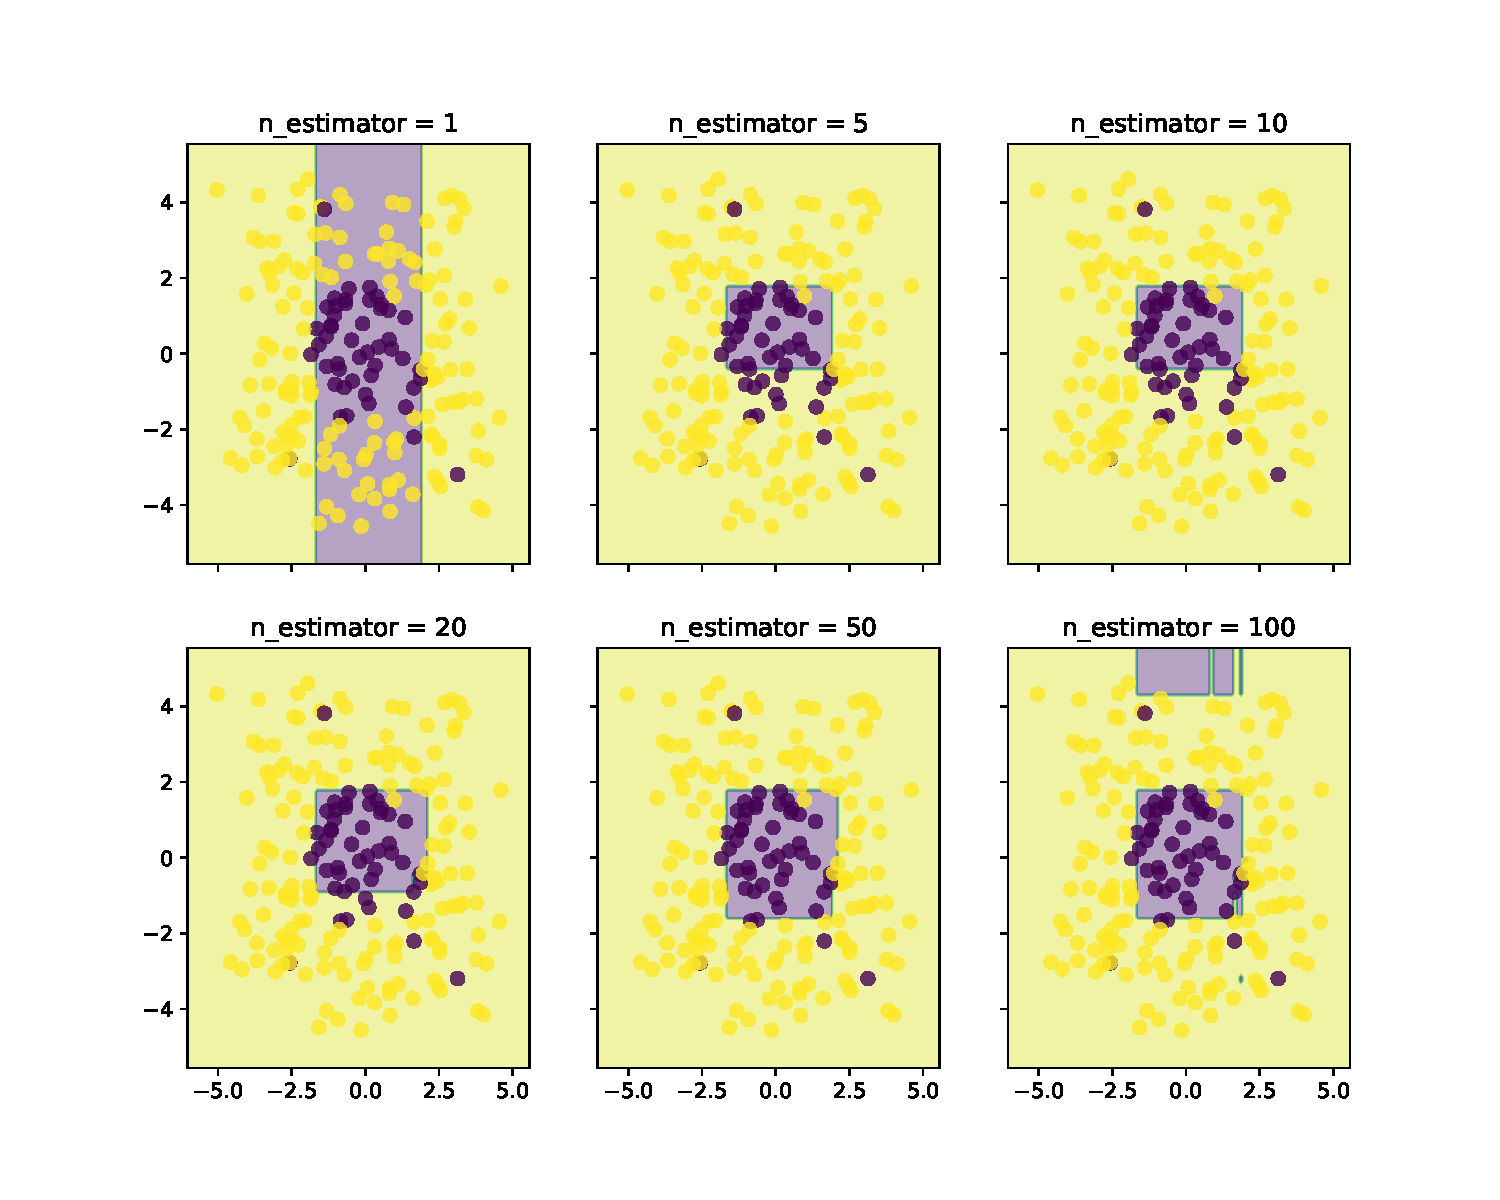
\includegraphics[width=.6\textwidth]{pdf/GBM_l2.pdf}
        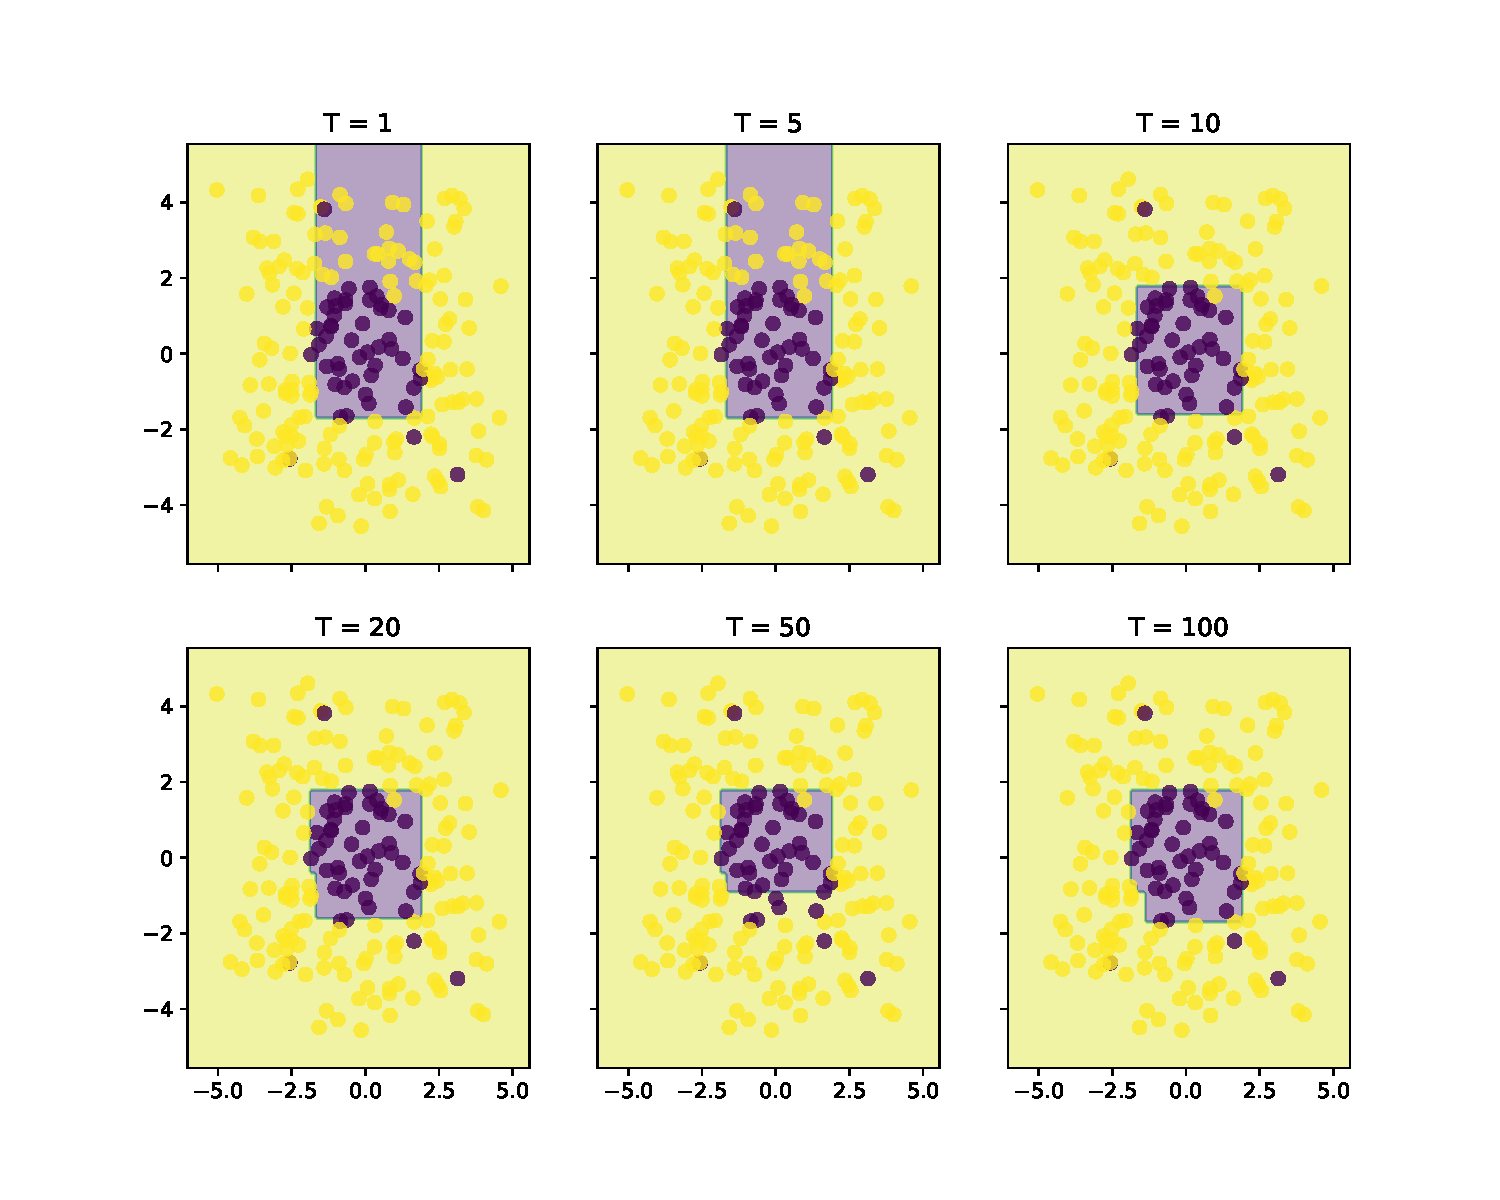
\includegraphics[width=.6\textwidth]{pdf/GBM_logistic.pdf}
        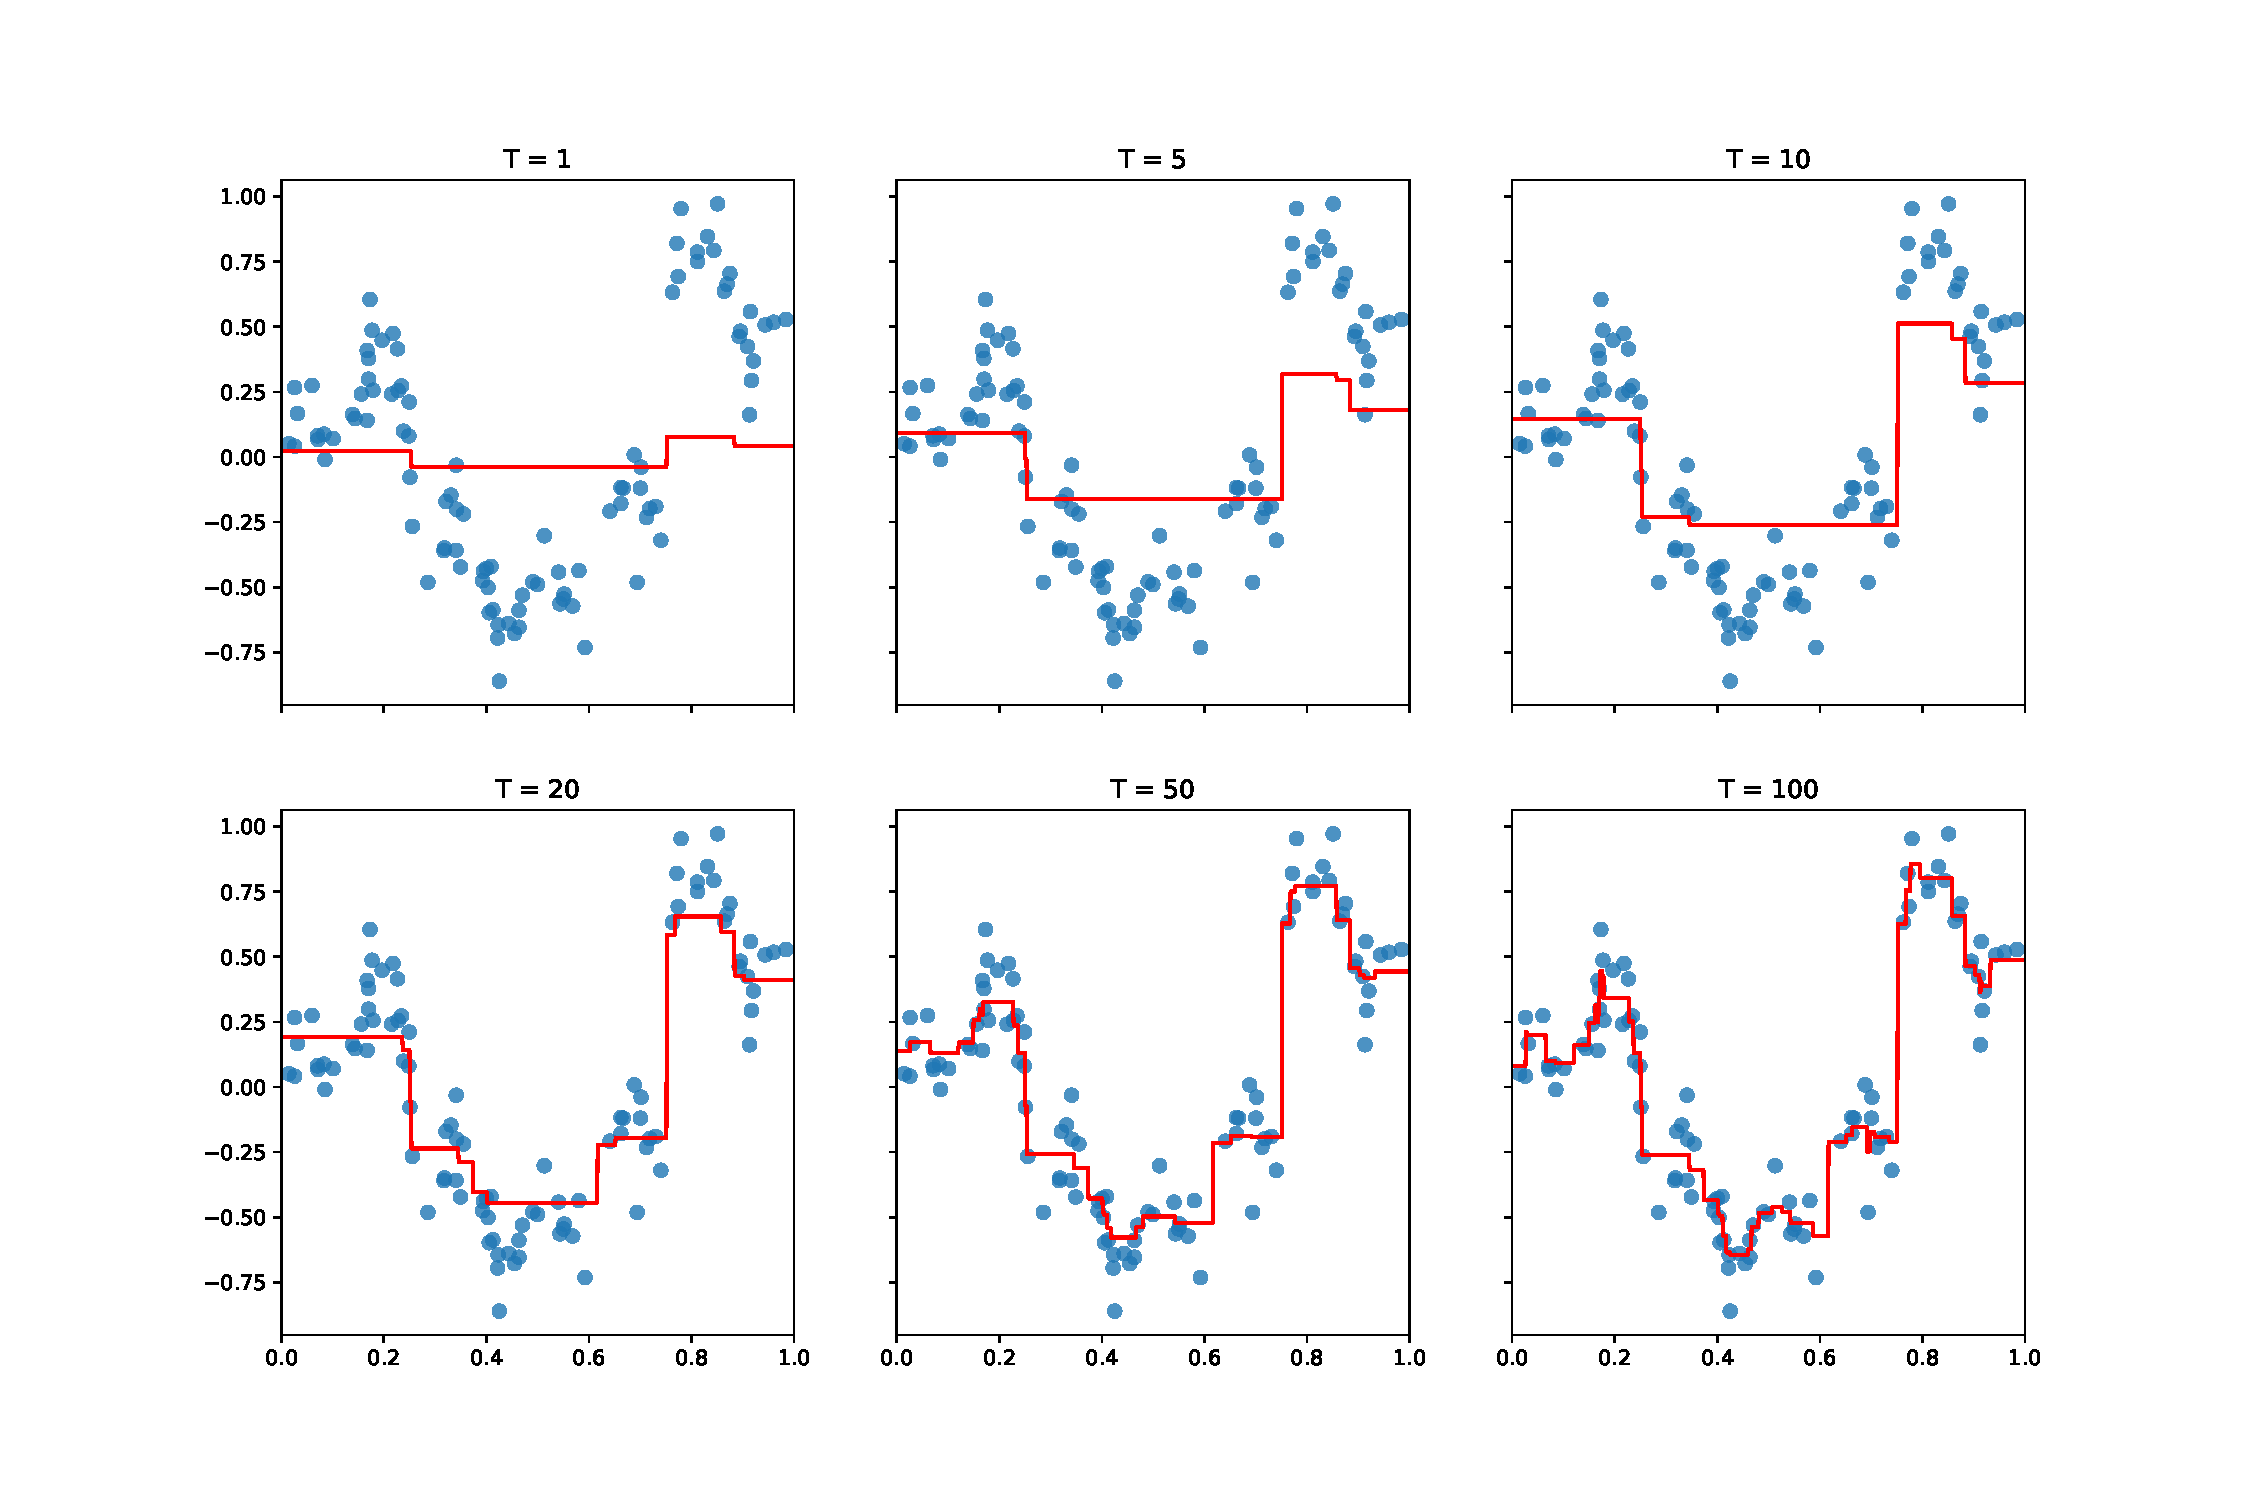
\includegraphics[width=.6\textwidth]{pdf/GBM_regression.pdf}
        \caption{Sol 3.5.7}
    \end{figure}
    
\end{solution}

\end{document}